\subsection{Modalanalyse (omega, modeshape, måling med mobil/frequency, FFT)} 

Modalanalysen inngår som en del av studien av konstruksjoners dynamiske egenskaper og oppførsel. Begrepet henger følgelig tett sammen med det overordnet temaet ``structural dynamics'', eller konstruksjonsdynamikk på norsk. Med egenskaper menes her egenfrekvenser, dempingskoeffisienter og modeformer (engelsk: \emph{mode shapes}). I påfølgende underkapitler skal vi introdusere kort om egenfrekvenser og modeformer.

\subsection{Egenfrekvenser}
For å forklare hva som menes med egenfrekvenser (flertall) til en konstruksjon, bør vi starte med å forklare hva én egenfrekvens (entall) er. En vanlig måte å introdusere dette på er å tegne opp en enkel konstruksjon som kun har èn frihetsgrad \parencite{CE809_FreeVibrationResponseOfSDFSystems}. Vi kaller konstruksjonen enkel fordi den ``\emph{..can be idealized as a concentrated or lumped mass \emph{m} supported by a massless structure with stiffness \emph{k} in the lateral direction} \parencite[s. 3]{Chopra2019-da}. I dette tilfelle en en-etasjers bygning med et voldsomt betongtak. Bygget er innspent mot bakken, og all massen antas altså å være plassert/konsentrert på taket. På figur \ref{fig:Enkel idealisert konstruksjon: én frihetsgrad} tenkes massen konsentrert i den blå sirkelen. At den har én frihetsgrad betyr her at det kun tillates én forskvyning/rotasjon. Her får forskvyningen $u$ gå langs aksen $x$:

\begin{figure}[h]
    \centering
    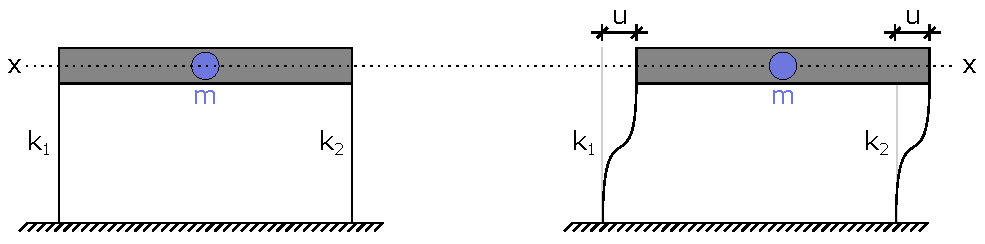
\includegraphics[width=\linewidth]{0 FIGURER/SDOF.pdf}
    \caption{Enkel idealisert konstruksjon: én frihetsgrad}
    \label{fig:Enkel idealisert konstruksjon: én frihetsgrad}
\end{figure}